
%
%   This file is part of the APS files in the REVTeX 4 distribution.
%   Version 4.0 of REVTeX, August 2001
%
%   Copyright (c) 2001 The American Physical Society.
%
%   See the REVTeX 4 README file for restrictions and more information.
%
% TeX'ing this file requires that you have AMS-LaTeX 2.0 installed
% as well as the rest of the prerequisites for REVTeX 4.0
%
% See the REVTeX 4 README file
% It also requires running BibTeX. The commands are as follows:
%                                                               /Users/neelimamgupte/Desktop/iitm.eps                                                                                                                                                                                 
%  1)  latex apssamp.tex
%  2)  bibtex apssamp
%  3)  latex apssamp.tex
%  4)  latex apssamp.tex
%
%\documentclass[twocolumn,showpacs,preprintnumbers,amsmath,amssymb]{revtex4-1}
\documentclass[preprint,showpacs,preprintnumbers,amsmath,amssymb]{revtex4-1}

% Some other (several out of many) possibilities
%\documentclass[preprint,aps]{revtex4-1}
%\documentclass[preprint,aps,draft]{revtex4}
%\documentclass[prb]{revtex4-1}% Physical Review B
\usepackage{graphicx}% Include figure files
\usepackage{dcolumn}% Align table columns on decimal point
\usepackage{bm}% bold math
\usepackage{amsmath,empheq}
\usepackage{hyperref}
\usepackage{natbib}
\newcommand{\overbar}[1]{\mkern 1.5mu\overline{\mkern-1.5mu#1\mkern-1.5mu}\mkern 1.5mu}


\begin{document}
\title{A mechanism to control synchronization in coupled area-preserving maps}
\affiliation{Department of Physics, Indian Institute of Technology Madras, Chennai, 600036, India.}
\author{Swetamber Das}
\email{swetdas@physics.iitm.ac.in}
\affiliation{Department of Physics, Indian Institute of Technology Madras, Chennai, 600036, India.}
%\author{Neelima Gupte}
%\email{gupte@physics.iitm.ac.in}
%\affiliation{Department of Physics, Indian Institute of Technology Madras, Chennai, 600036, India.}

\begin{abstract}
\pacs{05.45.+b}
\end{abstract}
\maketitle

\section{Introduction} 
Low-dimensional Hamiltonian systems commonly exhibit mixed phase space i.e. regular structures and chaotic regions may co-exist at a given degree of nonlinearity. This mixed nature has interesting consequences for the transport properties of such systems, for instance, the existence of anomalous kinetics, L\'{e}vy processes and L\'{e}vy flights \cite{Klafter1994,Zaburdaev2015}, power law contributions to recurrence and other statistics, and the existence of dynamical traps \cite{Zaslavsky2002a,Zaslavsky2002b}. An interesting region of a mixed phase space is the interface between regular regions and chaotic sea \cite{Mackay1984, Easton1993}. The dynamics in these neighbourhoods are complex and not well understood \cite{Meiss2015}. The complexity arises from the fact that a chaotic trajectory spends an arbitrary long but finite time at the boundaries of regular islands before exiting to the chaotic sea. The intermittent tendency of chaotic trajectories to stay close to the regular boundaries is called the phenomenon of stickiness. A major consequence of the stickiness is  the existence of power law in the Poincar{\'e} recurrence times indicating algebraic decay for long times times rather than exponential decay expected for normal transport. Therefore, due to stickiness, even a small regular island can influence the global transport properties of the system and decay of correlations. The phenomenon has been of great interest and continues to be studied on theoretical level \cite{Altmann2006, Altmann2010,Livorati2012,Bunimovich2012, Kruger2015}. In addition, stickiness has found application in several problems such as particle advection in fluids \cite{Babiano1994,Tel2005}, transport in plasma fusion devices \cite{Szezech2012,Martins2014}, celestial mechanics \cite{Efthymiopoulos1999, Harsoula2010, Harsoula2016}.

A recent feature of stickiness has emerged from a connected quarter. In our recent work~\cite{Mahata2016}, we have looked at the effects of the mixed phase space on the synchronization in a system of two standard maps coupled in unidirectional drive-response configuration. We have shown that synchronization of chaotic trajectories of the drive and response maps typically occurs in the neighborhood of regular inlands as a consequence of stickiness in the region.  This is the first instance, as far as we are aware, where stickiness have been found to influence synchronization in coupled chaotic systems.  For a chaotic orbit, synchronization typically happens via an intermittent behavior in the phase difference of the drive and response maps.   The sticky neighbourhoods of a regular islands contain Dynamical traps in chaotic orbits. In such trapping regions in the phase space, parts of a chaotic trajectory are almost regular in time and allow for synchronization to occur. Such traps are characterized using the properties of the finite-time Lyapunov exponent \cite{Szezech2005}. In the context of our work, we will refer to these traps as synchronization traps. We further noted that the behavior of the synchronization traps can be analyzed in a more quantitative way by analyzing the location and stability properties of the periodic orbits in the vicinity of the locations where synchronization takes place. 

Synchronization in coupled chaotic systems, coupled map lattices and networks 
have been studied in great details over the years. The fact however remains 
that the ability to control synchronization based on the dynamics of the 
process has not been given much attention, until 
recently~\cite{Grabow2011,Wang2016}. In realistic systems, the speed of 
processing of visual or  synchronization may be significant. For example, in 
neurosciences,  the speed of the visual and olfactory processing are 
interesting problems \cite{Thorpe1996,Uchida2003}. In this paper, we intend 
to develop a couple of 
mechanisms to control synchronization process to wit,  to increase and to 
decrease synchronization time based on the location of synchronization traps 
in the sticky neightborhood of regular islands in the phase space of the 
area-preserving system of the standard map. We demonstrate the mechanism at $K 
= 6$ where only two small regular islands exist.  The rest of the paper is 
organized in the following way: we explain the coupling scheme in 
sec.~\ref{sec:Pecora_Carroll}, the mechanism and demonstration of delay and 
advanced synchronization times in sec.~\ref{sec:delay} and 
sec.~\ref{sec:advanced} respectively, and the paper ends with conclusions in 
sec.~\ref{sec:conclusions} including discussion on limitations and 
implications. 


\section{The Pecora Caroll's unidirectional coupling scheme}
\label{sec:Pecora_Carroll} 
The standard map is considered to be the prototypical example of a two-dimensional area-preserving map, and is given by:

\begin{empheq}[right=\empheqrbrace \mod 1]{align}
P_{n+1} = P_n +  \frac{K}{2\pi}\sin(2\pi Q_n) \nonumber\\
Q_{n+1} = P_{n+1} + Q_n 
\end{empheq}

\begin{figure}[b]
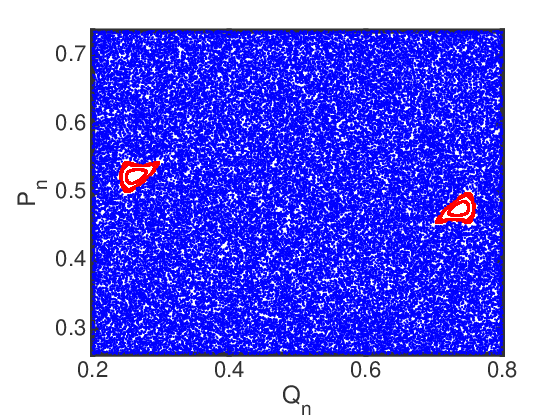
\includegraphics[scale=.6]{Standard_Map}
\caption{\label{fig:Standard_map} \footnotesize The phase space of the standard map for  random initial conditions from the uniform distribution on $[0,1]$,  at the parameter value K = 6.0.}
\end{figure}
Here the subscript $n$ denotes the discrete time and $K$ is the nonlinearity parameter. These equations typically describe the evolution of two canonical variables $P$ and $Q$ which correspond to the momentum and co-ordinate in the Poincar\'{e} section of a freely moving rotator with interleaved periodic kicks. This system represents the behavior of a variety of systems such as charged particle confinement in  mirror magnetic traps, particle dynamics in accelerator, comet dynamics in solar systems etc.  Two-dimensional  phase space plots  of the standard map for the parameter value $K = 6$ using $25$ initial conditions  are shown in Figs.~\ref{fig:Standard_map}.


We now synchronize two standard maps, using the Pecora-Carroll scheme of synchronization using drive-response coupling \cite{Pecora1990,Pecora2015}. 
This system was first devised to synchronize the chaotic trajectories dissipative chaotic dynamical systems. Under this unidirectional coupling scheme, we duplicate the given map and couple the original and the duplicated map in a drive-response configuration. This means that the drive map evolves freely but the evolution of the response map is dependent on the drive. In this case, the $P$ value of the response system is set to the $P$ value of the drive system, at each iterate.  Therefore, the coupled system is described by the following equations

\begin{minipage}[t]{0.5\textwidth}
\begin{empheq}[right=\empheqrbrace \mod 1]{align}\nonumber
\label{equ:drive}
P^d_{n+1} = P^d_n + \frac{K}{2\pi}\sin(2\pi Q^d_n)\nonumber\\
Q^d_{n+1} = P^d_{n+1} + Q^d_n \nonumber
\end{empheq}
\centering \textbf{(Drive)}

\end{minipage}
\begin{minipage}[t]{0.5\textwidth}
\begin{empheq}[right=\empheqrbrace \mod 1]{align}
P^r_{n+1} = P^d_n + \frac{K}{2\pi}\sin(2\pi Q^r_n) \nonumber \\
Q^r_{n+1} = P^r_{n+1} + Q^r_n \nonumber
\end{empheq}
\centering \textbf{(Response)}
\end{minipage}

\vspace{.5cm}

The initial values of $Q$ in the drive and response maps are chosen arbitrarily, whereas the $P$ values are identical. The system is said to reach complete synchronization when both the $Q$ values of the drive and response systems evolve asymptotically to identical values i.e. 
\begin{equation}
\lim_{t\rightarrow\infty}(Q^d_n - Q^r_n) = 0
\end{equation}

Synchronization time is the least value of the iterate say, $\tau$, where $\Delta Q = Q^d-Q^r$ vanishes and remains so for rest of the iterations. 
\begin{equation}
(Q^d_n - Q^r_n) = 0; \hfill  n \geq  \bf {\tau }
\end{equation}

In all of the computations reported in the work, two chaotic trajectories are considered to be synchronized to numerical accuracy, if the Euclidean distance between them is less than $10^{-5}$. An example is shown in Fig.~\ref{fig:sync_ex}. Here, we plot $\Delta Q = Q^d_n-Q^r_n$ for initial conditions $(P^d_0,Q^d_0,Q^r_0) = (0.569, 0.906,0.106)$ at $K = 6$. The synchronization time is found to be 570246. 

\begin{figure}[t]
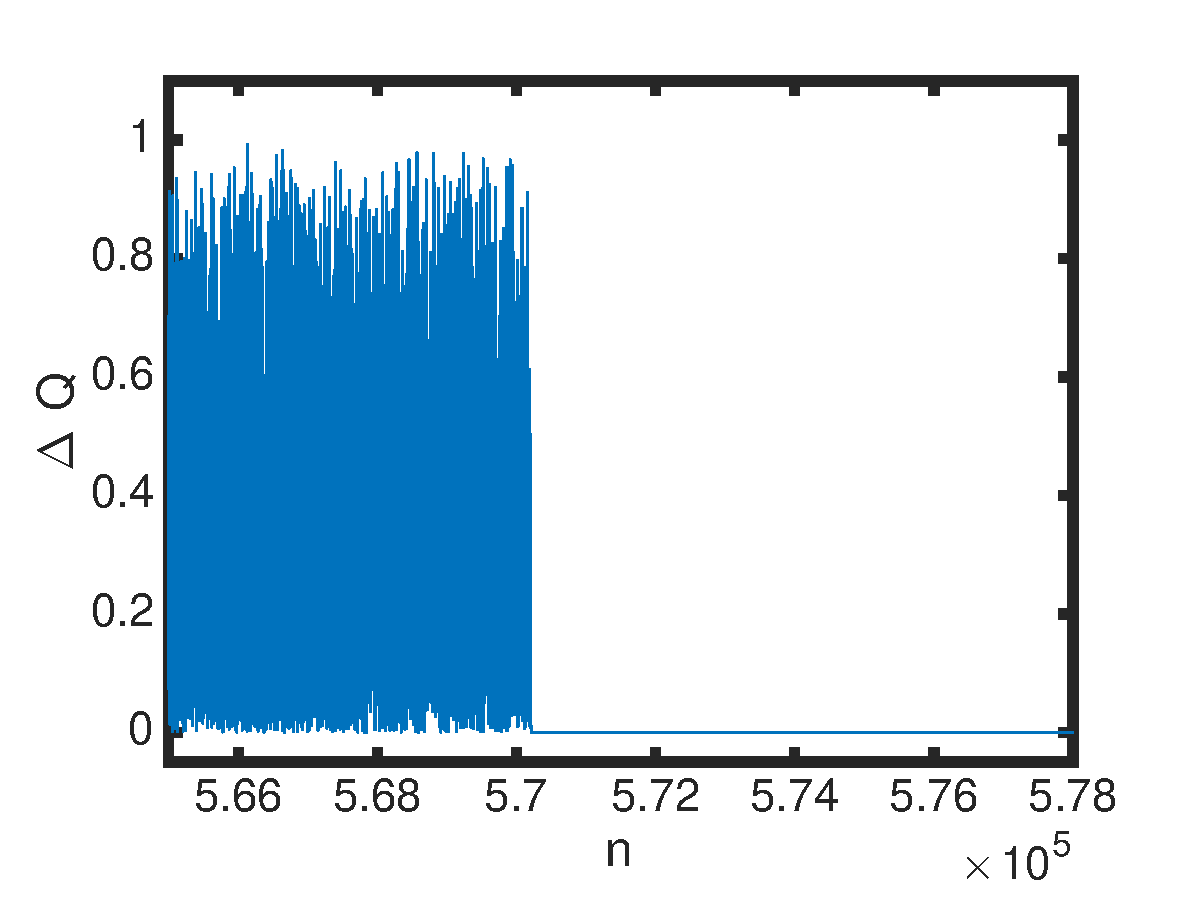
\includegraphics[scale=.6]{Sync_exmaple}
\caption{\label{fig:sync_ex} \footnotesize The variation of $\Delta Q = Q^d_n-Q^r_n$ of the coupled system at $K = 6$ with iterations $n$. Synchronization is considered to be achieved when $\Delta Q < 10^{-5}$ and remain so for the rest of the iterations. The iteration step $n$ at which synchronization occurs is called synchronization time $\tau$. For this case, $\tau = 570 246.$ }
\end{figure}

We now analyze synchronization of the coupled system using the master stability function~\cite{Pecora1998}. The numerical procedures to control synchronization times will be discussed thereafter.  

\section{Locating Synchronzation Traps using Master stability function}
\label{Master stability function}
A general drive-response system coupled unidirectionally may be described by the following set of equations

\begin{align}
\frac{d\overbar{X}_d}{dt} = \overbar{F}(\overbar{X}_d) \nonumber  &&
\frac{d\overbar{X_r}}{dt} = \overbar{F}(\overbar{X}_r) + \alpha E(\overbar{X}_d-\overbar{X}_r)
\end{align}

Here $\overbar{X}_d$ and $\overbar{X}_r$ are drive and response variables; the matrix $E$ determines the linear combination of the $\overbar{X}$ used in the difference and $\alpha$ is the coupling strength. For the map case, we have the following form

\begin{align}
\overbar{X}^d_{n+1} = \overbar{F}(\overbar{X}^d_{n}) \nonumber  &&
\overbar{X}^r_{n+1} = \overbar{F}(\overbar{X}^r_{n}) + \alpha E(\overbar{X}^d_{n}-\overbar{X}^r_n)
\end{align}

Therefore, in the case of a general unidirectional coupling of two standard maps, we get

\begin{center}
\begin{empheq}[right=\empheqrbrace \mod 1]{align}
P^d_{n+1} = P^d_n + \frac{K}{2\pi}\sin(2\pi Q^d_n) \nonumber\\
Q^d_{n+1} = P^d_{n+1} + Q^d_n \nonumber\\
P^r_{n+1} = P^r_n + \frac{K}{2\pi}\sin (2\pi Q^r_n) + \alpha(P^d_n-P^r_n) \nonumber \\
Q^r_{n+1} = P^r_{n+1} + Q^r_n 
\label{equ:coupled}
\end{empheq}
\end{center}

We have chosen $E$ to be the matrix $\begin{bmatrix} 1 & 0 \\ 1 & 0 \end{bmatrix}$. 

To find the stability of the synchronous state, we first express  Eq.(\ref{equ:coupled}) in terms of  $P^\perp = P^d - P^r$ and $Q^\perp = Q^d - Q^r$, as follows
\begin{eqnarray}
\label{equ:trans}
P^\perp_{n+1} = (1-\alpha)P^\perp_n+ \frac{K}{2\pi} \sin(2\pi Q^d_n) - \frac{K}{2\pi} \sin(2\pi Q^r_n) \\ \nonumber
Q^\perp_{n+1} = (1-\alpha)P^\perp_n+ Q^\perp_n + \frac{K}{2\pi} \sin(2\pi Q^d_n) - \frac{K}{2\pi} \sin(2\pi Q^r_n)  
\end{eqnarray}

We now write the variational equation for Eq.(\ref{equ:trans}) by linearizing about $(P^d_n,Q^d_n)$
\begin{equation}
\label{equ:variational}
\left[ \begin{array}{c} \delta P^\perp_{n+1} \\ \delta Q^\perp_{n+1} \end{array} \right] = \mathcal{M}(\alpha)\left[ \begin{array}{c}\delta P^\perp_{n} \\ \delta Q^\perp_{n} \end{array} \right]
\end{equation}
where the matrix $\mathcal{M}(\alpha)$ is given by
\begin{equation} 
\label{equ:M}
\mathcal{M}(\alpha) = \begin{bmatrix} 1-\alpha & K\cos(2\pi Q^d_n) \\ 1 - \alpha & 1 + K\cos(2\pi Q^d_n) \end{bmatrix} 
\end{equation}





This is the master stability equation for the unidirectionally coupled standard map. The variational equation (\ref{equ:variational}) is the master stability equation for the coupled system under investigation. The associated largest LE computed from the master stability equation is the master stability function of the system, given by:
\begin{equation}
\label{equ:msf}
\lambda  = \lim_{n \rightarrow \infty} \lim_{\delta\overbar{X}_0\rightarrow 0}\frac{1}{n}\sum^{n-1}_{i=0}\ln|JM^n(\overbar{X}_i)|
\end{equation}

Here $n$ is a positive integer and $JM^n(\overbar{X}_i)$ denotes the Jacobian matrix of the $n$-times iterated map.  A negative value of the MSF (the largest non-zero LE) will ensure that $(P^\perp,Q^\perp) $ tend to zero indicating that the difference between $P$ and $Q$ will die out and the system will synchronize. 
Now, for the Pecora-Carroll approach, we set $\alpha = 1$. This substitution simplifies the matrix in Eq.(\ref{equ:M}) which now reads

\begin{equation} 
\mathcal{M}(1)= \begin{bmatrix} 0 & K\cos(2\pi Q^d_n) \\ 0 & 1 + K\cos(2\pi Q^d_n) \end{bmatrix} 
\end{equation}

The MSF should then be computed from the eigenvalues of the matrix $\mathcal{M}(1)$. It is easy to see that, for $\alpha =1$, one of the eigenvalues of   $\mathcal{M}(1)$ is zero. Therefore, we need to consider only the non-zero eigenvalue which is $1+K\cos(2\pi Q^d_n)$. The corresponding LE is given by

\begin{equation}
\label{equ:LE}
\lambda   = \lim_{n \rightarrow \infty} \frac{1}{n}\sum^{n-1}_{i=0}\ln|1+K\cos(2\pi Q^d_n)|
\end{equation}

In general, we define the $kth$ time-$n$ Lyapunov exponent associated with an initial point $\overbar{X}_0 = (P_0,Q_0)$ for a map $M(P,Q)$ as
\begin{equation}
\label{equ:FLEf}
\lambda _k(\overbar{X}_0;n)  = \frac{1}{n}\sum^{n-1}_{i=0}\ln|JM^n(\overbar{X}_i)|
\end{equation}

\begin{figure}[h]
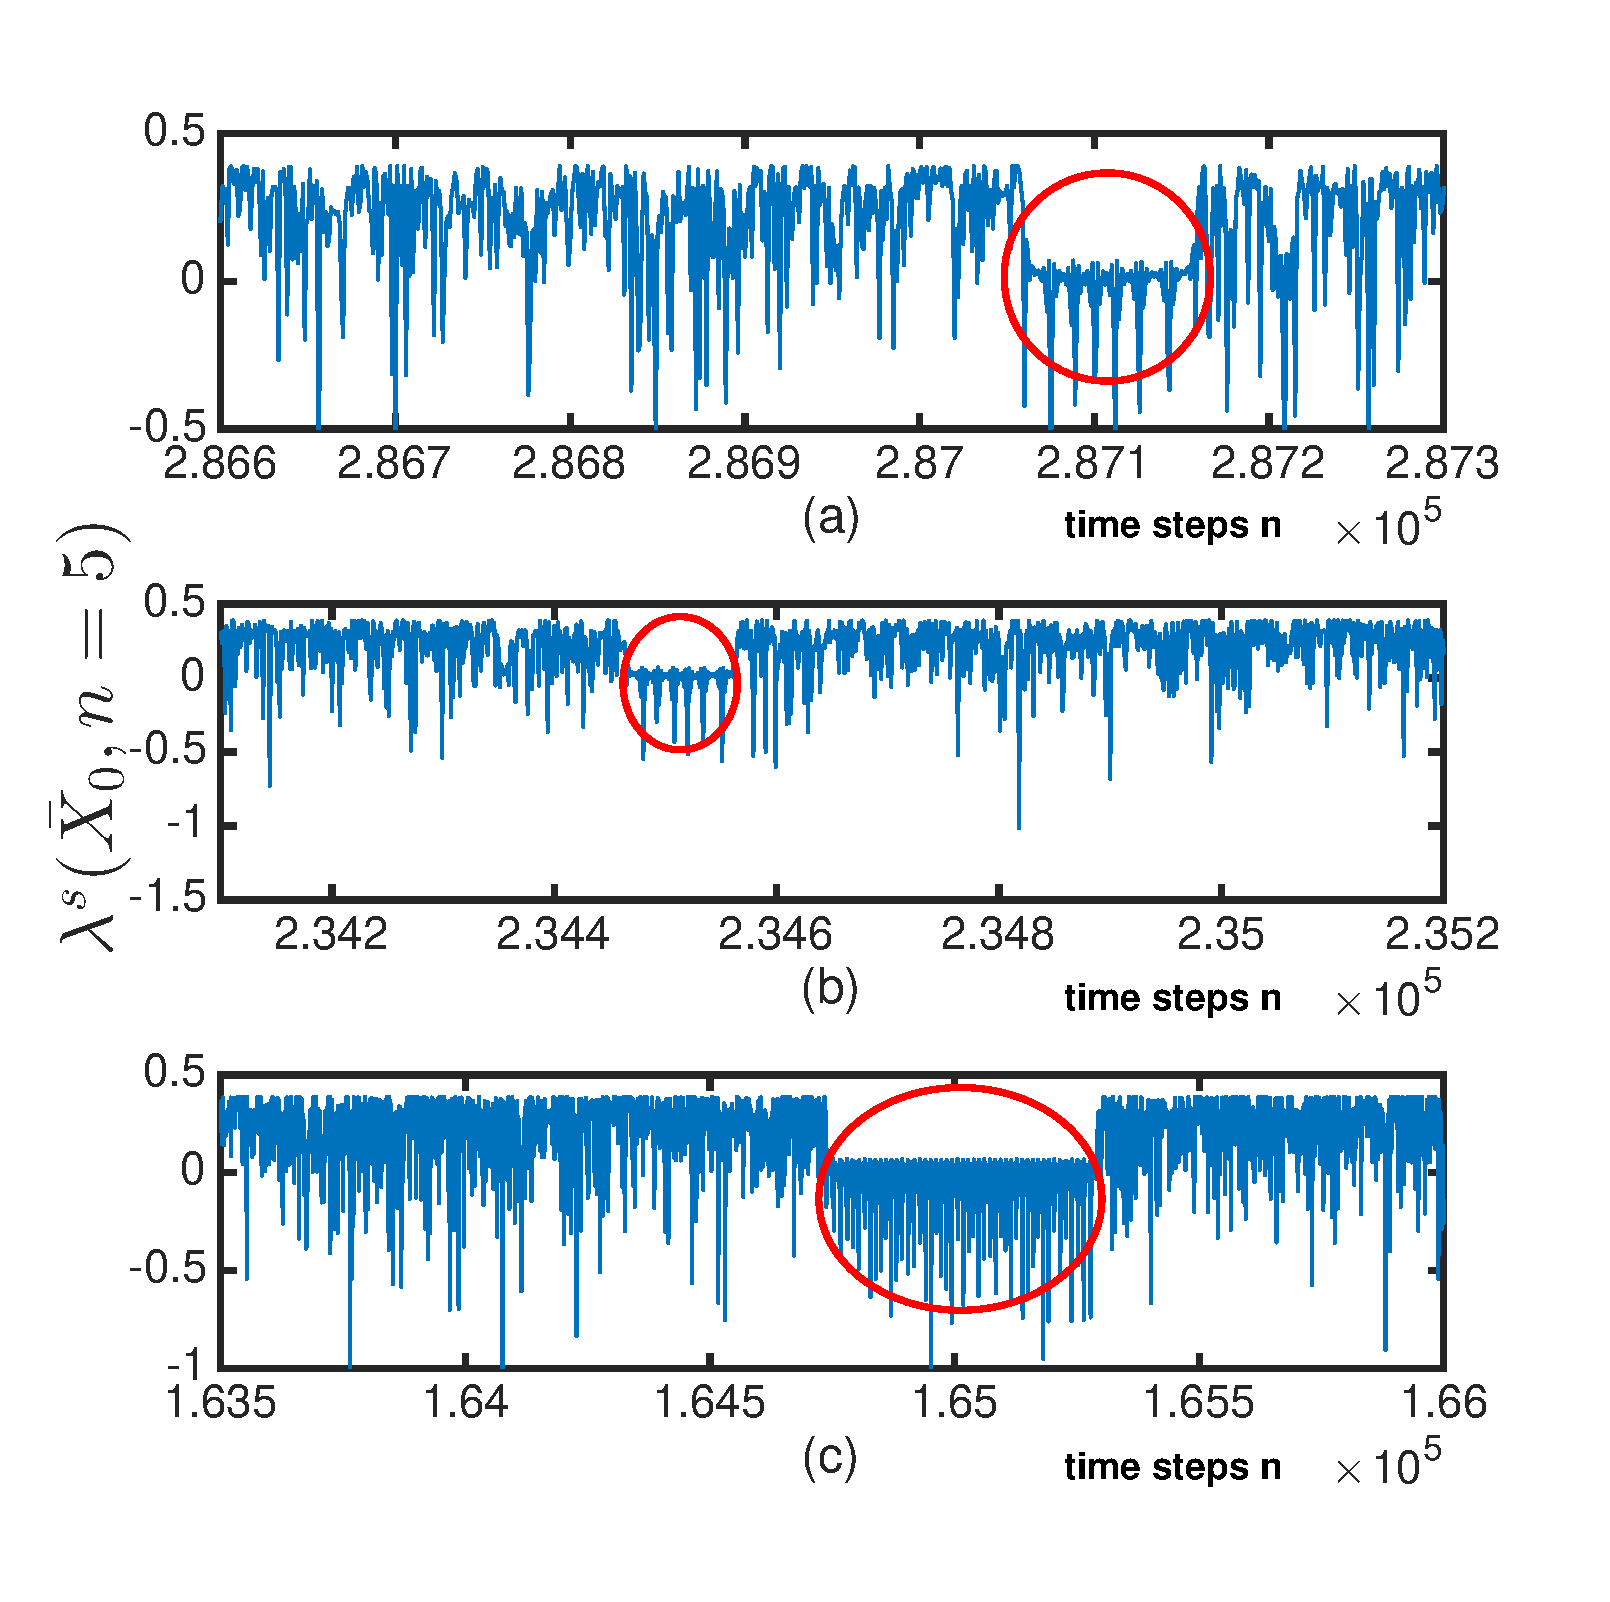
\includegraphics[scale=0.55]{FTLE_plots}
\caption{\label{fig:FTLE}\footnotesize Fluctuations of time-5 FTLEs for three different set of initial conditions -- $(P^d_0,Q^d_0,Q^r_0) = (0.466,0.098,0.141)$ in (a),  $(0.009,0.026,0.129)$ in (b), and $(0.553,0.554,0.396)$ in (c). The synchronization times in each cases are 287090, 234521, and 164782 respectively. The time scale on the x-axis indicates iterates steps $t$ at which time-5 FTLEs have been computed. The drop window in (a), (b), and (c) shown in ellipses in red occur around synchronization times. Synchronization of chaotic trajectories in the coupled system under study typically occurs in one of such traps.}
\end{figure}


Here $n$ is a positive integer and $JM^n(\overbar{X}_i)$ denotes the Jacobian matrix of the $n$-times iterated map. We extend this notion to the master stability function defined in the Sec.~\ref{Master stability function}  i.e.  the non-zero Lyapunov exponent defined in Eq.(\ref{equ:LE}) 
which takes the following finite time version 
\begin{equation}
\lambda_1^s(\overbar{X}_0;n) = \frac{1}{n}\sum^{n-1}_{i=0}\ln|1 + K \cos (2\pi Q_i)|
\end{equation}

The subscript ($k = 1$) has been dropped hereafter as we have only one LE to compute.

We plot the variation in the time-5 FTLE defined above at $K = 6$. At the point of synchronization, the FTLE values attain a set of negative values consistently in a small window, indicating the existence of a synchronization trap.  In Fig.~\ref{fig:FTLE} , the three plots show the fluctuations  of FTLE near the point of synchronization for three different sets of initial conditions - $(P^d_0,Q^d_0,Q^r_0) = (0.466,0.098,0.141)$ in (a),  $(0.009,0.026,0.129)$ in (b), and $(0.553,0.554,0.396)$ in (c) with synchronization times 287090, 234521, and 164782 respectively. The values on the x-axis indicate time steps at which averages are computed so that synchronization times and the temporal neighborhood are effectively captured in the plots wherein a temporary drop is clearly visible, indicated by ellipses in red. Synchronization of chaotic trajectories typically occurs in one of such traps. 

\section{Delayed Synchronization Times}
\label{sec:delay}
In order to develop a numerical technique to delay synchronization, we  first have to identify the vicinity of regular islands in the phase space. Another mechanism  to suppress stickiness based on knowledge of hyperbolic and non hyperbolic regions in the phase has been reported recently~\cite{Kruger2015}. Our method, however, targets the trajectories themselves in the sticky region to delay the process. We employ the edge-detection algorithm due to Benkadda {\it et al.} \cite{Benkadda1997}. For the numerical procedure, we divide the phase space in $100 \times 100$ grid. The edges of both the islands are detected by applying the standard map to point initiated in the chaotic sea, for $10^7$ times.  The edges thus detected in shown in Fig.  We have chosen the thickness parameter to be $d = 0.02$ i.e. euclidean distance of $d$ from points on the edge indicate the extent of the vicinity of the island.  This vicinity, therefore, indicate the the domain wherein the synchronization traps exist.  To demonstrate this explicitly, we compare the phase angles, defined by $\theta = \tan^{-1}\frac{Q}{P}$, of the points on the numerically detected edges and the points of synchronization, as follows. 

In Fig.~\ref{fig:Edge_Sync_angles}(a), we show the distribution of phase angles of the points on the edges of regular islands determined by the edge-detection algorithm.  The bimodality of the distribution is due to the existence of two sharp islands in otherwise chaotic bulk in the phase space.  We compare this with the phase angles corresponding to the points in the phase space at which synchronization of the chaotic trajectories occurs.


\begin{figure}[h]
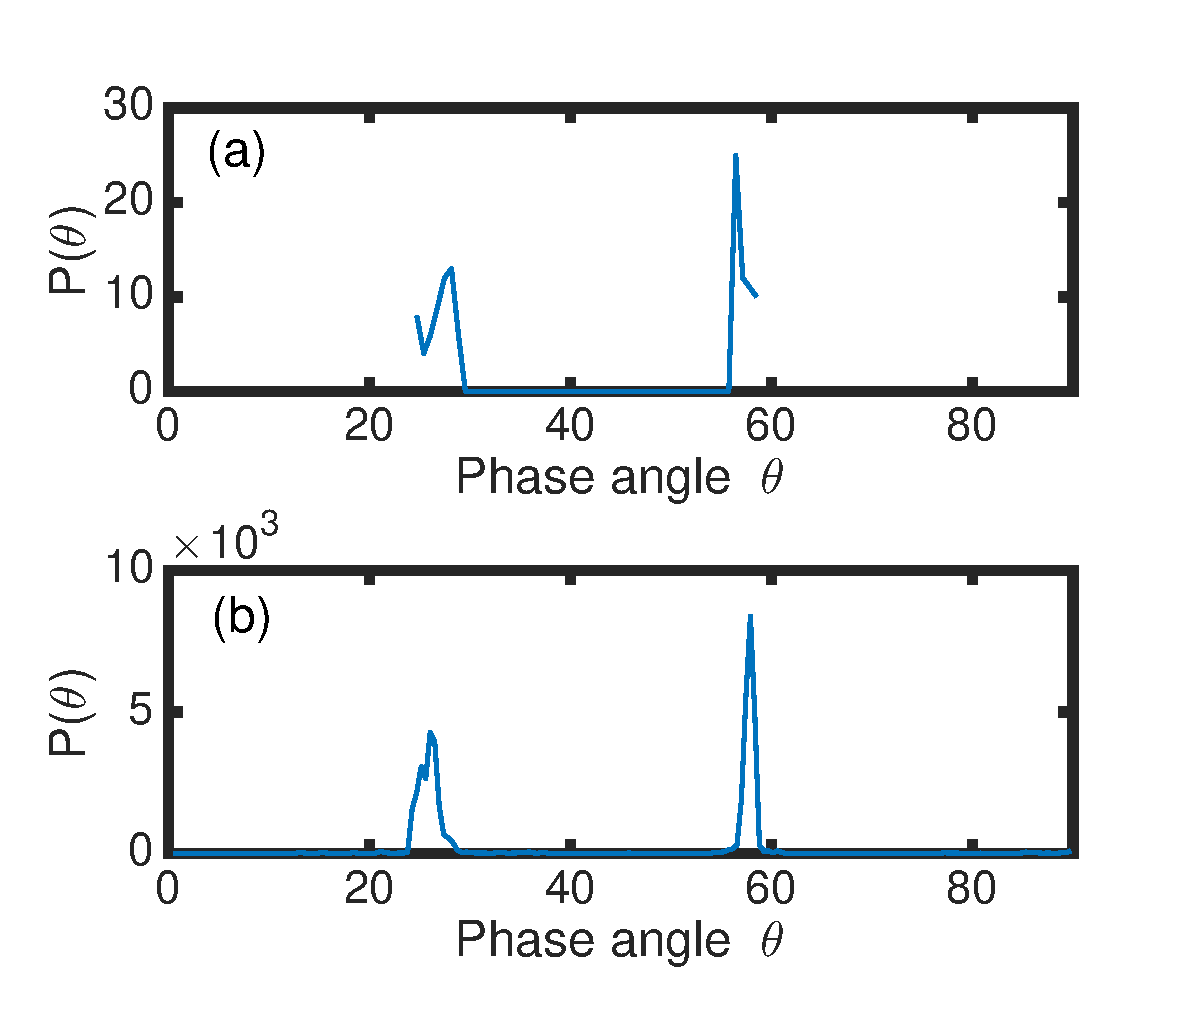
\includegraphics[scale=0.6]{Edge_Sync_angles}
%\includegraphics[scale=.4]{Standard_Map2.eps}\\
\caption{\label{fig:Edge_Sync_angles} \footnotesize Numerical detection of 
synchronization traps (a) Distribution of phase 
angles of the points on the edges of regular islands determined by the edge 
detection algorithm. (b) Distribution of phase angles for points where 
synchronization occurs. }
\end{figure}

Fig.~\ref{fig:Edge_Sync_angles}(b) shows the distribution of these phase angles for about 50 000 randomly chosen initial conditions for the drive and response maps that lead to synchronization. The locations of the peaks in the distribution shown in (a) approximately matches with this in (b). It is, therefore, visibly clear that synchronization occurs in the same angular domain of the phase space where the regular islands exist. Our numerically detected edges, thus correctly locate the synchronization traps in the phase space.  We now discuss the control mechanism to delay synchronization time. 

The proximity parameter $d_0 = 0.02$ defines the region in the neighbourhood of the numerically detected edges wherein synchronization traps exist. The basic idea to control synchronization time is to identify the step at which the chaotic trajectory visits the numerically determined sticky neighbourhood followed by a slight deflection so that the trajectory resters at a point outside.  Our procedure depends upon how many times we deflect the trajectory  which will be referred to as step control. This means that if an $n-$step control is  employed then, the trajectory will be kicked away from the domain $n$-times during its first $n$ visits i.e. once per visit. The deflection is achieved by adding a randomly generated fraction below $0.1$ to the point visiting the domain, and therefore the maximum deflection area is roughly $1\%$ of the phase space.  This procedure applied on a given set of initial conditions of the drive and response maps, may result in four possibilities of synchronization time -- (1) successful delay  \textbf{(S)}, (2) no delay \textbf{(N)}, (3) failed to achieve synchronization \textbf{(F)}, and (4) undesirable faster synchronization \textbf{(U)}. Clearly, the only first possibility is the aim of the mechanism; the last one constitute a hazard while the other two are trivial. 
\begin{figure}[h]
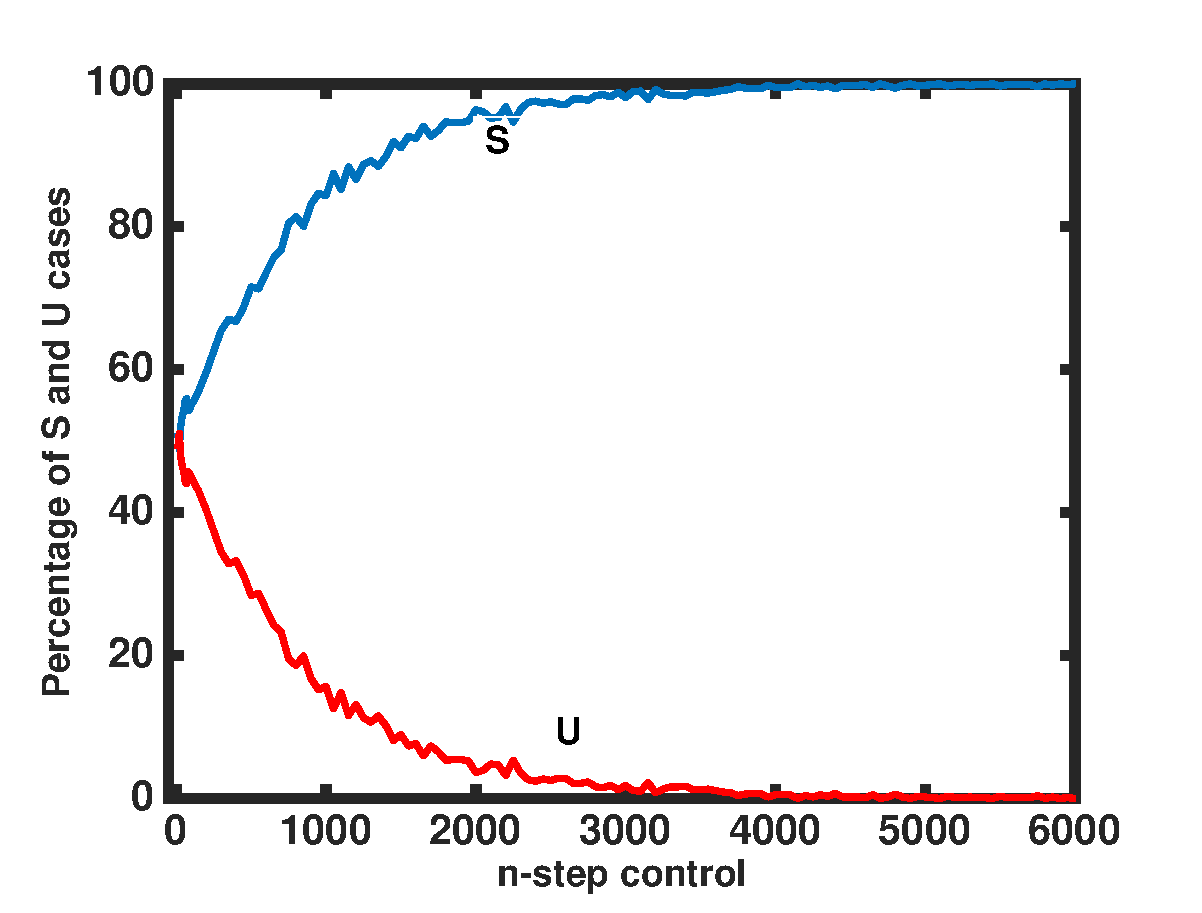
\includegraphics[scale=0.6]{S_U_Percent}
\caption{\label{fig:Control_success} \footnotesize. The curves indicate the 
percentages of (S) successful delays shown as the blue curve,a and (U) 
undesirable fast synchronization showns as the red curve. }
\end{figure}

For the numerical implementation of the mechanism, we have considered $1000$ randomly chosen initial conditions from the chaotic sea of the phase space at $K = 6$. The maps have been iterated for $10^7$ times in each case.  The sticky domain is the determined by the proximity parameter $d_0$ around the numerically detected edges of the regular islands. We demonstrate the effectiveness of the control procedure  with respect to several $n-$step controls. The computations have been performed for $n \in \mathbb{A}$, where $\mathbb{A} = \{10, 20,30,...,90, 100, 150, ... ,10 000\}$.  

\begin{figure}[t]
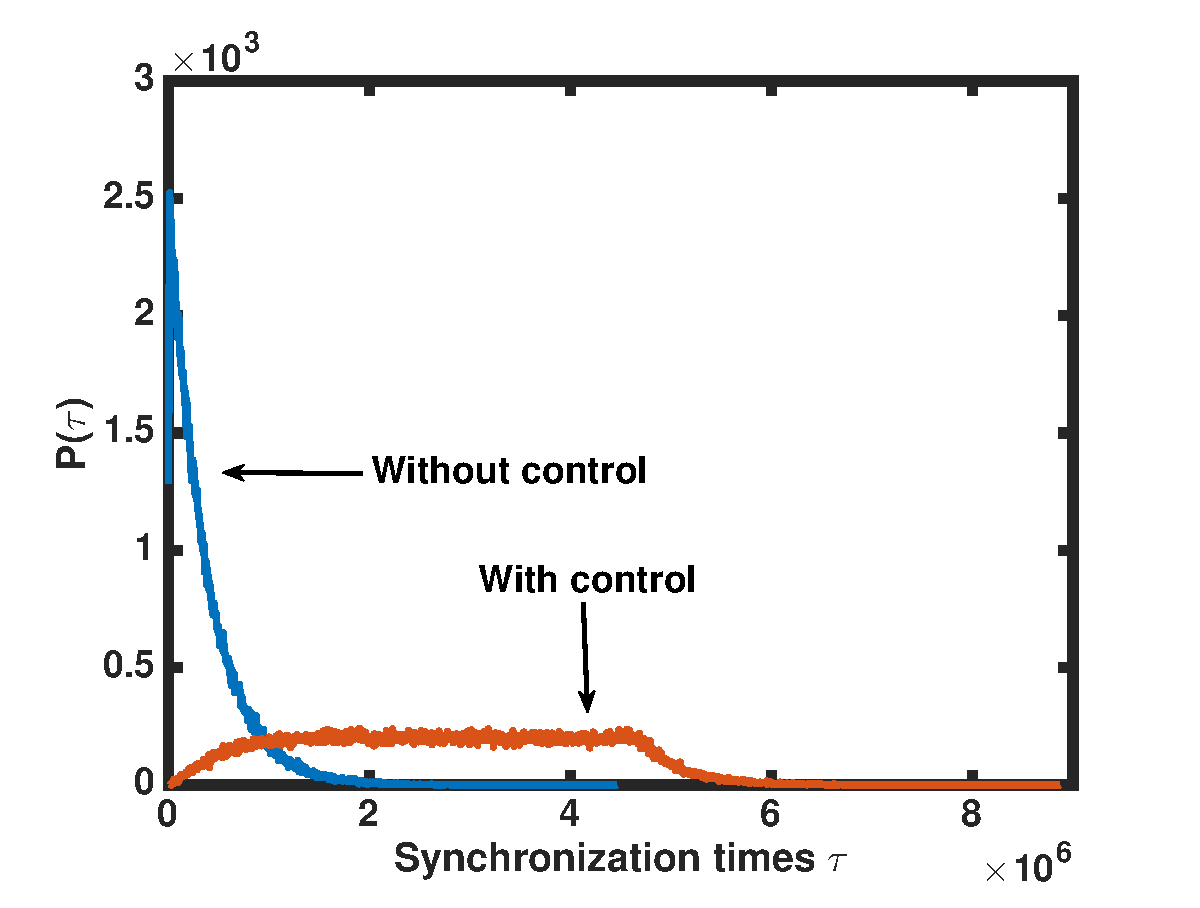
\includegraphics[scale=0.6]{Sync_time_dist.eps}
\caption{\label{fig:Sync_time_dist} \footnotesize. Distribution of 
synchronization time without n-step control (the blue curve) and with n-step 
control (the red curve). The control delays synchronization times. }
\end{figure}


Fig  shows the percentage of successful delays \textbf{(S)} (on the y-axis) for a given $n-$step control (on the x-axis) up to $n = 5500$ after which the successful cases are always $100\%$.  We achieve about $50\%$ successful cases for $n = 10$, which rises rapidly to $99\%$ for $n = 2950$. It is to be noted that the average synchronisation time without any control, $\tau_{avg} \sim 10^5$. Therefore, the n-steps required to obtain all successful delays is just about $3\%$ of $\tau_{avg}$. We also plot the distribution of synchronization times for successful cases and compare it against that of corresponding times without control in Fig. The long-tailed distribution of times without delay crosses over to a distribution which shows large flat region before a tail. The flat region indicate large number of successfully applied control with typical delay times of the order of $10^6$. For complexness, we show the decay in the number of undesired cases \textbf{U} in Fig.  The cases \textbf{F} and \textbf{N} which are largely present for $n<10$, are extremely small in number and are neglected. 


 \begin{figure}[t]
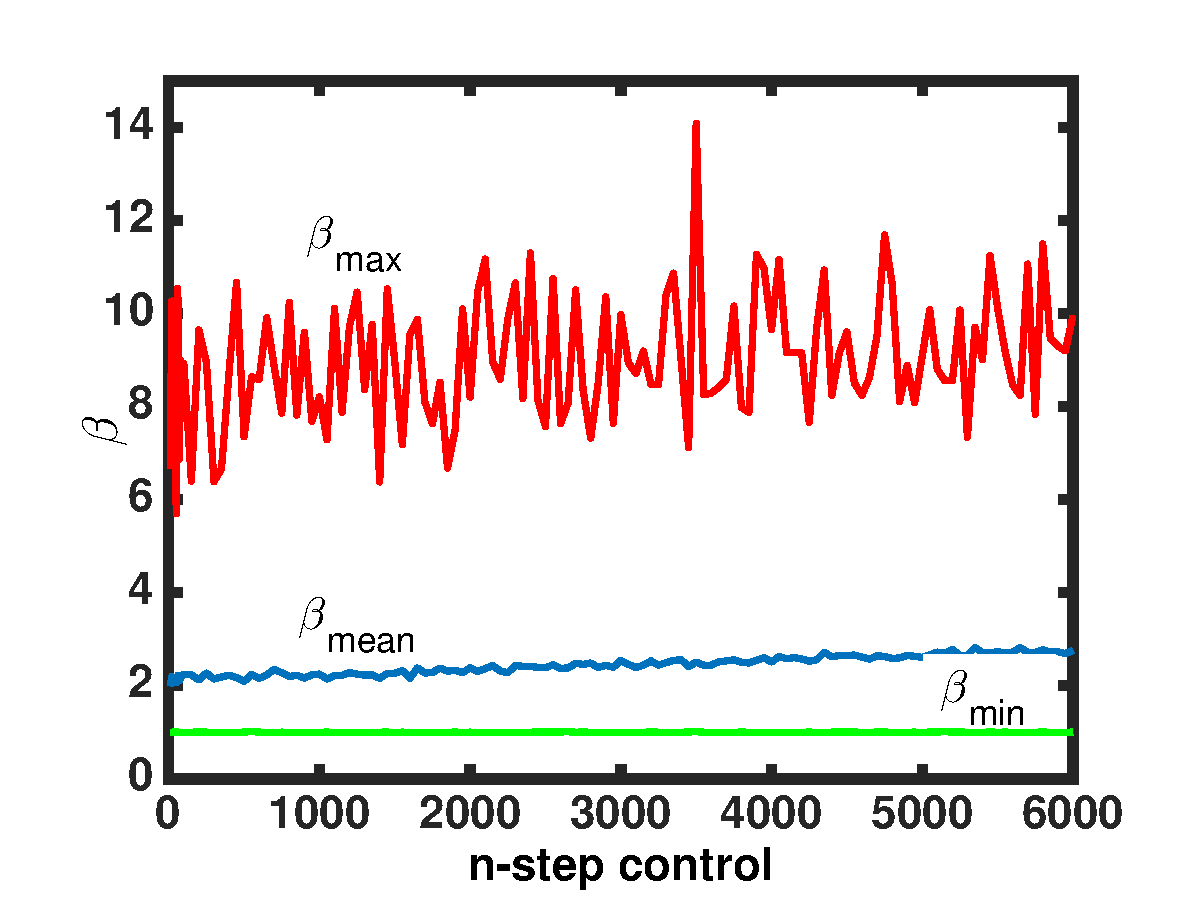
\includegraphics[scale=0.6]{Strength_con.eps}
\caption{\label{fig:Strength_con} \footnotesize. Variation of $\beta$ 
(maximum, minimum and average) which measures the strength of successful 
delays i.e. $\beta = \ln(\frac{\tau_d}{\tau_0}$. $\beta_max$ indicates the 
maximum delay time obtained at a give n-step control while $\beta_{mean}$ 
stands for the mean value around 2. This means that on an average, 
synchronization times re delayed by 100 times. The minimum value of $\beta$ 
remains 1 for the cases when no delay was obtained obtained. }
\end{figure}


  The extent of delay $\beta$ may be defined as the ratio of successfully 
  delayed synchronization times $\tau_c$ to synchronization times $\tau_0$ 
  without control, i.e. $\beta =  \ln(\frac{\tau_d}{\tau_0}$).  Therefore, for 
  successfully delayed synchronization $\beta>0$ indicating $\tau_c > \tau$. 
  The plot in Fig.~\ref{fig:Strength_con} shows the variation of $\beta$ i.e. 
  $\beta_{min}$, $\beta_{mean}$, and $\beta_{max}$  indicating minimum, mean 
  and maximum $\beta$ for considered $n-$step controls. Clearly, we are able 
  to attain $\beta_{max}$ values to be in the range $5$ to $14$ while mean 
  values remain $\sim2$. Therefore, we are successful in achieving 
  significantly large delays in synchronization times. 
  





There are a couple of limitations of the proposed control procedure. The deflection to the trajectory visiting the sticky domain should not insert it inside the regular island. The regular trajectories of the drive and response map are known to synchronize significantly faster and would result in the undesirable possibility \textbf{(U)}. Therefore, an estimate of the size of regular islands, in addition to their locations must be known. These may be determined efficiently, as we have shown, using the edge-detection algorithm. The deflection area  may then be chosen suitably.  Another limitation is that the procedure is unable to impose a pre-determined delay to synchronization times. The random deflections simply keep the trajectories temporarily away from the synchronization traps in the sticky domain and synchronization may eventually occur after the removal of the control. 

 
 \section{Advanced Syncronization Times}
 \label{sec:advanced}
 We now explore the possibility to decrease synchronization times i.e. to expedite the process of synchronization. Once again, we will make use of the fact that synchronization traps typically exist in the sticky neighbourhoods of the regular islands.  The procedure is based on the parameter perturbation technique to generate coherent structures in the phase space of an area-preserving map. However, the technique may also be used to push the chaotic bulk on the coherent structure (regular region) already present in the phase space and therefore, to make it disappear completely.  We describe the procedure briefly. 
 
 In a given area-preserving map, for instance, the  standard map, a  perturbation in the nonlinearity parameter $K$ in the neighbourhood of a suitable chosen periodic point leads to generation of large coherent structure.   We take the same form the standard map with a modulo operation such that $-0.5 \leq P_n \leq 0.5, 0\leq Q_n \leq 1$ . In the form above \cite{FN1}, the standard map is known to have a hyperbolic fixed point at $(0,0)$,$(0,0.5)$. We perturb the parameter $K$ to $K-\epsilon$ if $|P - P_f| < \delta$, $|Q-Q_f| < \delta$. For $P$ and $Q$ outside this $\delta$-strip, $K$ does not change.  It may be noted that the perturbed standard map remains to be area-preserving. The Jacobian $J$ is now given by: 
 
\begin{minipage}[t]{0.55\textwidth}
%\raggedleft
\centering
\[ J = \left( \begin{array}{cc}
1 & 1 + (K-\epsilon)\cos(2\pi Q_n)   \\
1 & (K-\epsilon)\cos(2\pi Q_n) \end{array} \right)\]  
\end{minipage}
\begin{minipage}[t]{0.4\textwidth}
\raggedright

\vspace{0.65cm}
$ \epsilon \neq 0$ if $|P_f - P_n| < \delta$, $|Q_f - Q_n| < \delta$\\ $\epsilon = 0$, otherwise.\\
\end{minipage}

\vspace{0.65cm}
The determinant of this matrix $J$ remains 1. The phase space thus obtained for for $K = 6$ , $\delta = 0.3$ and $\epsilon = 2$ for the fixed point $(P_f,Q_f)=(0.0,0.0)$ is shown in Fig.~\ref{fig:coherent}.   We have performed computation for the other fixed point and with other modulo operations as well and results do not differ significantly. Our choice here of modulo operation and the fixed point $(P_f,Q_f)$ has some advantage over the others in terms of actual numerical values of synchronization times and the display of locations of the points where synchronization occurs. 
 
For the computations, we take 50 000 initial conditions chosen randomly from the chaotic region of the unperturbed standard map.  The procedure has been applied to both drive and response map in accordance with our coupling  scheme described above. We choose a patch around $(P_f,Q_f)$  of length $\delta= 0.3$ which corresponds to about $9\%$ of the phase space area. We successfully obtain advance synchronization in more that $99.5\%$ of the cases among which a  couple of instances  has been shown in Fig.~\ref{fig:location} wherein synchronization occurs in the neighbourhood of the main regular island and one of its satellite islands.  The sign `+' in red indicate the point of synchronization. 
 \begin{figure}[h]
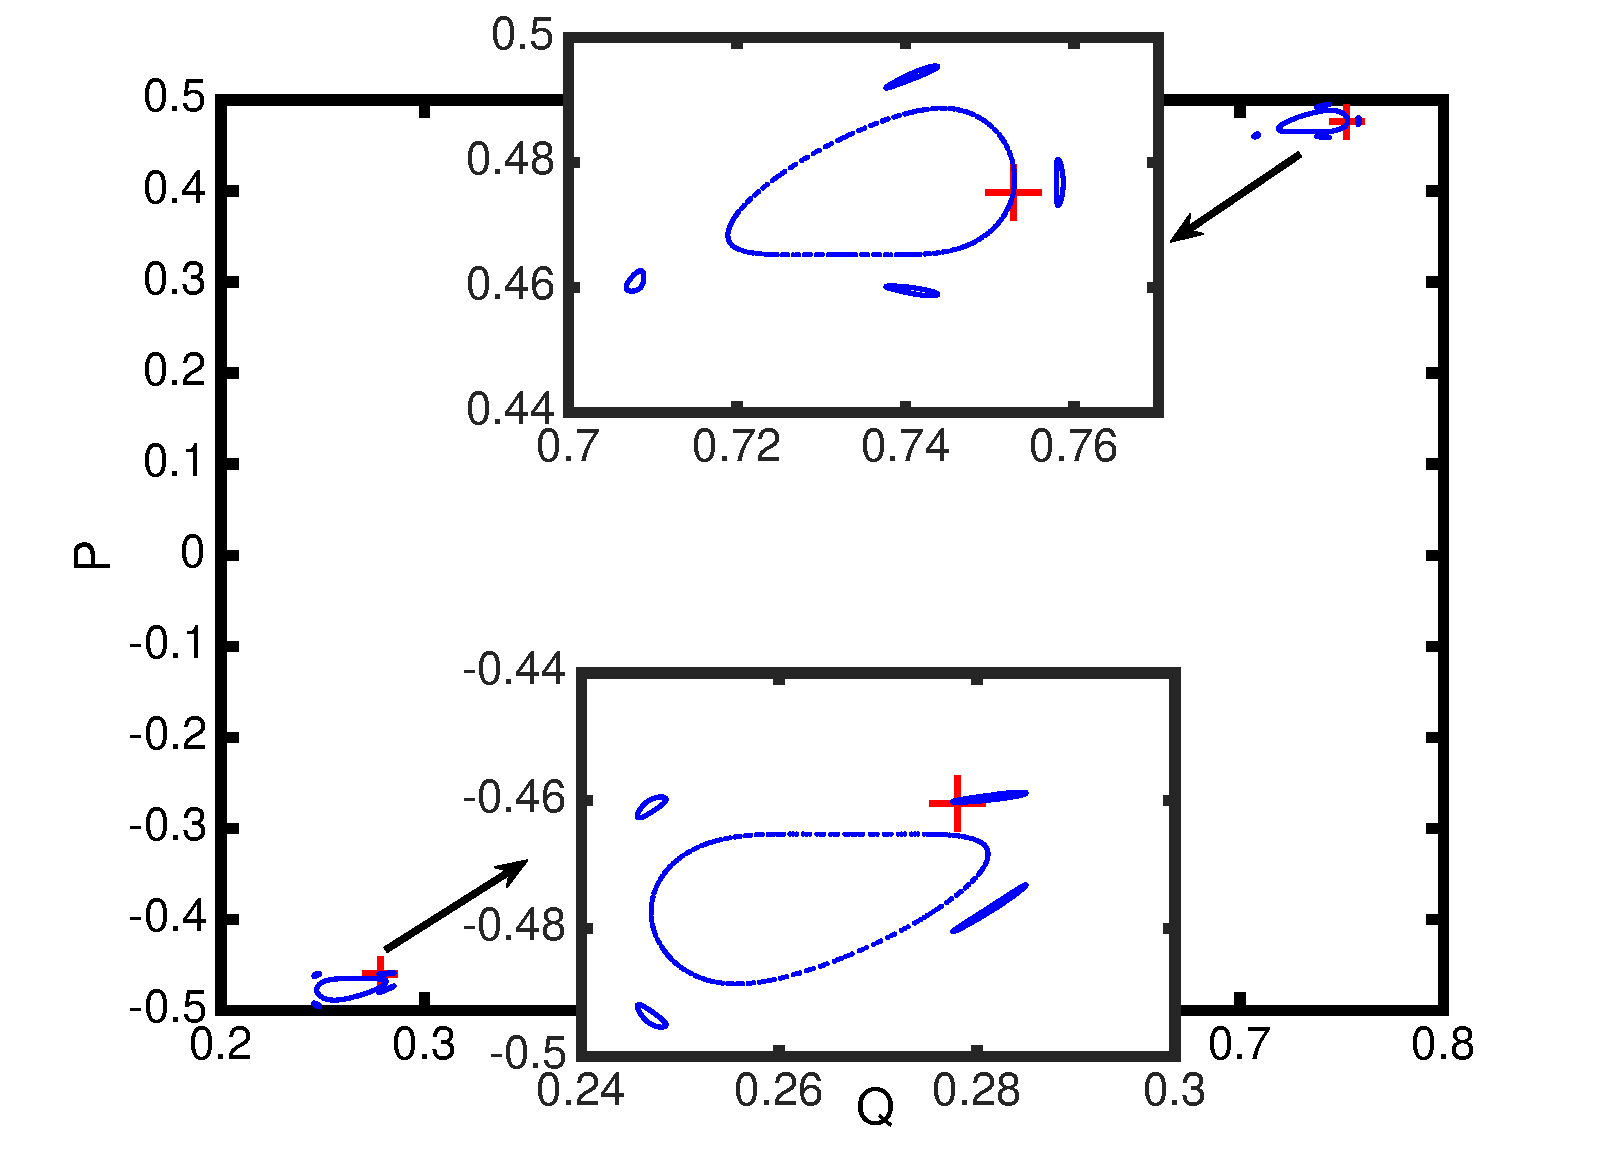
\includegraphics[scale=0.6]{Fast_sync_location.eps}
\caption{\label{fig:location} \footnotesize.The phase space of the drive map 
at K = 6 where parameter perturbation is applied. Synchronization occors at 
the location indicate by the red 'plus' signs.}
\end{figure}
 
 \begin{figure}[h]
\begin{tabular}{cc}
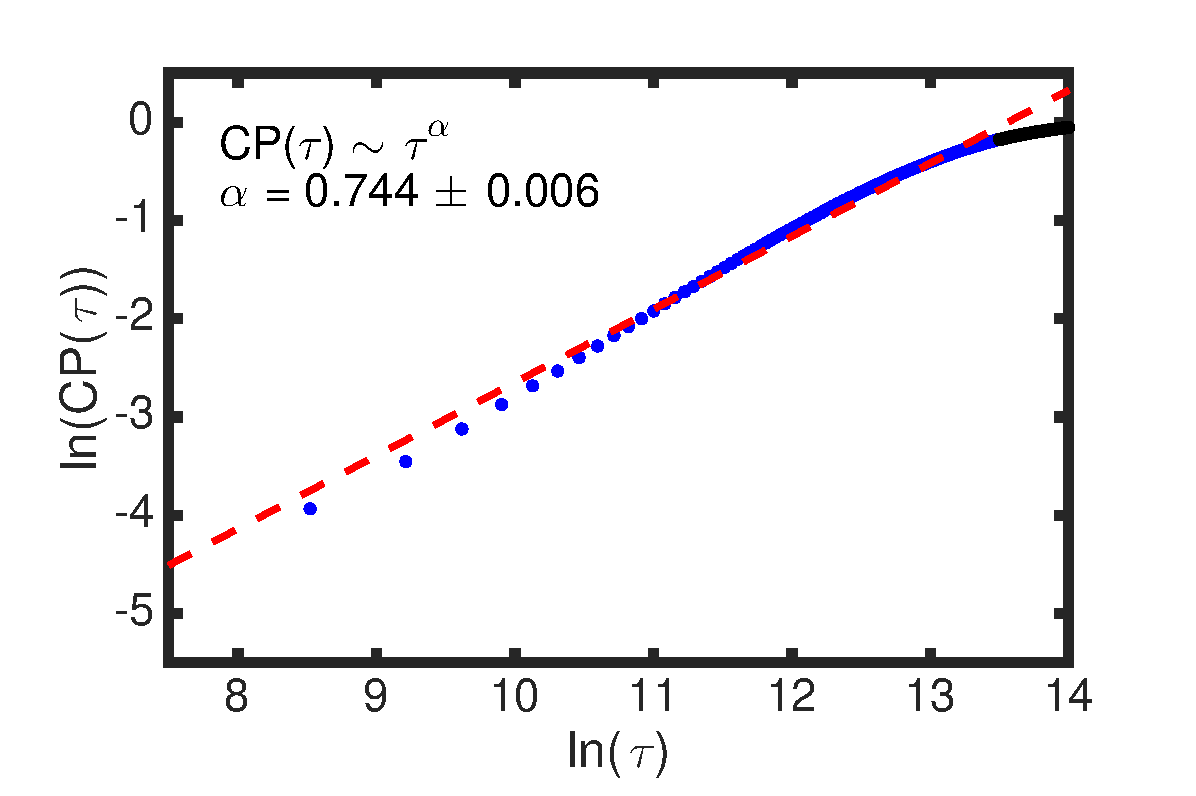
\includegraphics[scale=0.45]{Normal_Sync.eps}&
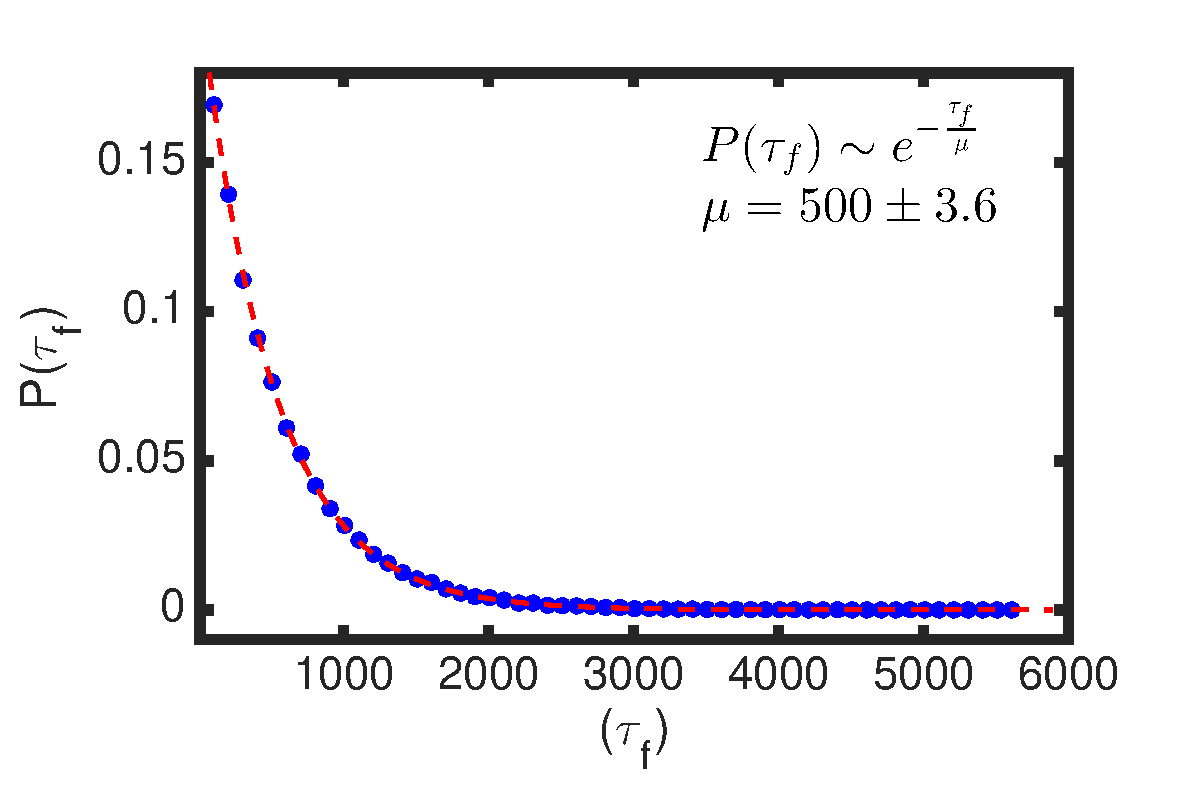
\includegraphics[scale=0.45]{Fast_sync_dist.eps}\\
(a) & (b)
\end{tabular}{}
\caption{\label{fig:sync_time_dist} \footnotesize The phase space of the standard map for 25 random initial conditions from the uniform distribution on $[0,2\pi]$ plotted for 4500 iterations; 500 iterates are discarded as transients. The values are normalized i.e. $\frac{P}{2\pi} $ and $\frac{Q}{2\pi}$ are plotted on the $y$ and $x$ axis for the parameter values (a)  K = 1.5, and (b) K = 6.0.}
\end{figure}

The probability distribution of synchronization times without parameter perturbation shows a long tail which shows a power law scaling. It is shown using cumulative probability distribution on a log-log scale in Fig.~\ref{fig:sync_time_dist}(a) with slope $\sim 0.744$. Upon application of perturbation, synchronization times become considerable shorter and the probability distribution cross over to exponential. Fig.~\ref{fig:sync_time_dist}(b) shows the resulting exponential distribution for the same set of initial conditions as shown for in Fig.~\ref{fig:sync_time_dist}(a) , with an estimated mean $\sim500$. Comparing the $x-$scales of the plots, one can see the faster synchronization has been successfully achieved.  

We again define the strength of controlled synchronization as $\beta = \ln \frac{\tau_c}{\tau}$. For advanced synchronization, $\beta < 0$ indicating that synchronization times upon parameter perturbation is smaller than in normal course i.e. $\tau_c < \tau$. The probability distribution of $\beta$ in shown in Fig.~\ref{fig:beta_dist}, which may be fit with a gaussian of the following form:
\begin{equation}
f(\beta) =  a\exp(-\frac{(\beta-\mu)^2}{2c^2})
\end{equation}

We estimate the mean value $\mu \sim - 6.648$ and standard deviation $\sigma \sim1.542$ which corresponds to the fact that, on an average, advanced synchronization times thus obtained are $4\times10^2$ times smaller than the normal synchronization times with $95.5\%$ values are between $10$ to $10^4$ times smaller.  Therefore, the synchronization times we obtained upon parameter perturbation is significantly smaller than the normal synchronization times.  

The parameter perturbation technique is an efficient way to decrease synchronization times with high accuracy.  The value of the perturbation imposed should be chosen suitably as a very small may not have any influence on the synchronization process. The procedure also depends on the size and location of the patch wherein the control is applied. We are yet to see if the other technique of generating coherent structures also influence synchronization in these unidirectionally coupled systems. 


 \begin{figure}[h]
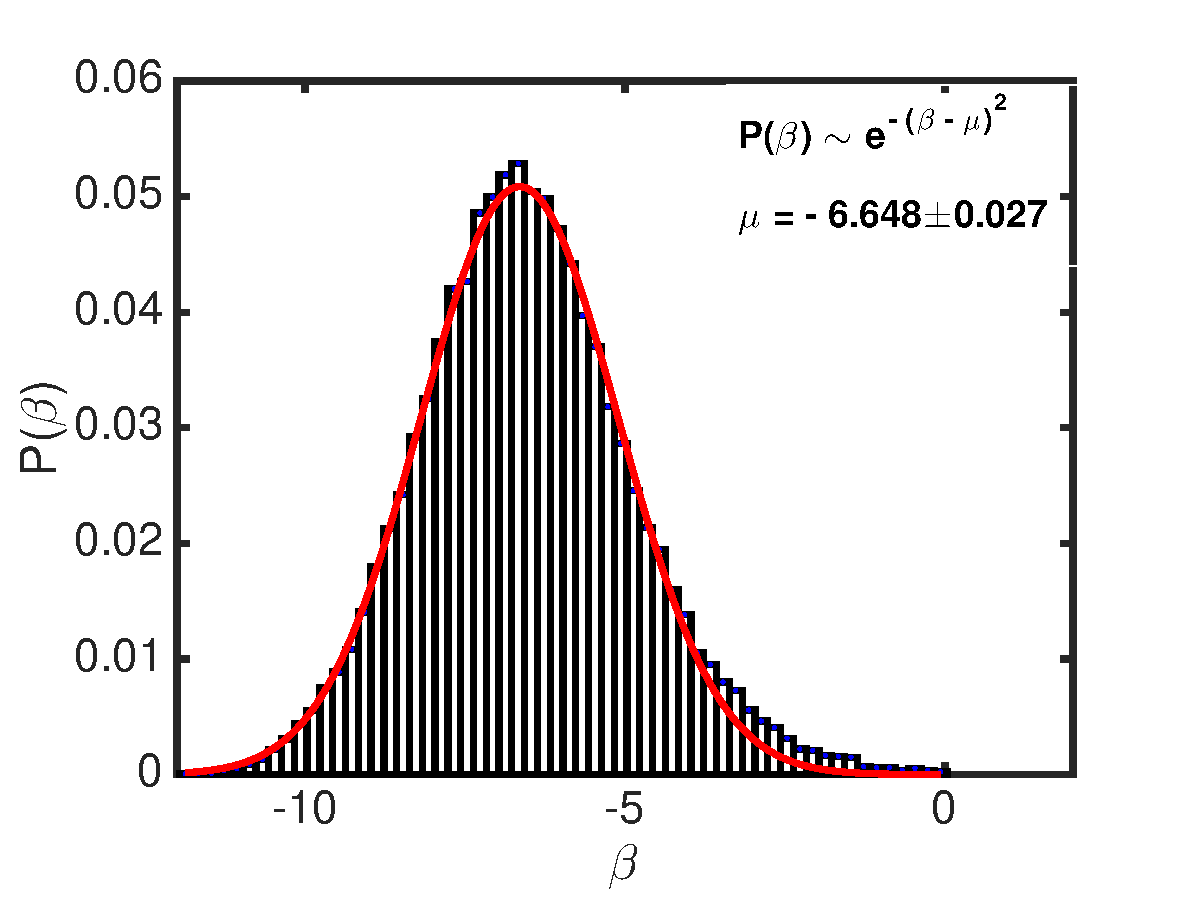
\includegraphics[scale=0.6]{Fast_strength_dist.eps}
\caption{\label{fig:location} \footnotesize.}
\end{figure}
 
\section{Conclusions}
\label{sec:conclusions}
To summarise, we have developed a numerical procedure to delay synchronization in two identical standard map coupled under the drive-response configuration. The procedure is based on the fact that synchronization in the system typically occurs in the sticky neighbourhoods of the regular islands in the phase space. We have shown that the delay is obtained by kicking the trajectories slightly away from the domain temporarily. The efficiency of the procedure depends upon the number of steps employed in control. By applying the procedure to the system on merely $1\%$ of the phase space area (at $K = 6$), we have successfully increased synchronization times. The maximum number of control steps that are used is $0.01\%$ of the total of number of iterations used throughout the computation.  Furthermore, the procedure gives variety of delays. The limitations of the procedure are, one, the deflection may insert the drive trajectory in the regular islands which would lead to undesirable faster synchronization and two, a predetermined synchronization time in not obtainable. 

%\begin{thebibliography}
\bibliographystyle{unsrt}
\bibliography{Syncref} 

%\end{thebibliography}
\end{document}



